\begin{figure}[h]
  \centering
  \includegraphics[width=5cm]{./Cbillard_1.pdf}
  \caption{Interprétation du $\alpha$ de la vitesse initiale}
  \label{fig: Cbilliard_1}
\end{figure}

\begin{enumerate}
  \item \label{alphainit} Le réel $\alpha$ est un argument de $\frac{v_0}{z_0}$ donc une mesure de l'angle entre $\overrightarrow{OM_0}$ et $\overrightarrow{v_0}$ (fig \ref{fig: Cbilliard_1}). Le mouvement se fait \emph{à l'intérieur} du billard si et seulement si
\begin{displaymath}
  \alpha \in \left] \frac{\pi}{2} , \frac{\pi}{2} + \pi\right[ = \left] \frac{\pi}{2} , \frac{3\pi}{2}\right[.
\end{displaymath}
  \item En utilisant la définition de $\cos$ avec une exponentielle:
\begin{displaymath}
  1-2\cos\alpha e^{i\alpha} = 1-\left(e^{-i\alpha} + e^{i\alpha} \right)e^{i\alpha} =- e^{2i\alpha} = e^{i(2\alpha + \pi)}
\end{displaymath}

  \item \begin{enumerate}
\item Les points dont l'affixe vérifie la condition imposée forment la droite passant par $M_0$ et de direction $\overrightarrow{v_0}$.
\item \label{premchoc}Avec les conditions précisées par l'énoncé, on peut chercher l'affixe du premier point de contact avec le bord sous la forme $z_0 + \lambda z_0 e^{i\alpha}$ avec $\lambda$ réel non nul. Ce complexe doit être de module 1 ce qui donne $1+\lambda^{2}+2\lambda \cos\alpha =1$ donc $\lambda=-2\cos\alpha$. On en déduit 
\begin{displaymath}
z_1 = (1-2\cos\alpha e^{i\alpha})z_0 = -e^{2i\alpha}z_0 = e^{i(2\alpha - \pi)}z_0  
\end{displaymath}
De plus
\begin{displaymath}
  \frac{v_0}{z_1} = \frac{z_0 e^{i\alpha}}{z_0 e^{i(2\alpha - \pi)}} = e^{i(-\alpha + \pi)}
  \Rightarrow -\alpha + \pi \text{ est un argument de } \frac{v_0}{z_1}
\end{displaymath}
\end{enumerate}

\begin{figure}[h]
  \centering
  \subfloat[Choc élastique en $M_1$]{\label{fig:Cbillard_2} \includegraphics[width=4.5cm]{./Cbillard_2.pdf}} \hspace{1cm}
  \subfloat[Vecteurs en $M_1$.]{\label{fig:Cbillard_3} \includegraphics[width=4.5cm]{./Cbillard_3.pdf}}
  \caption{Question \ref{reflex}}
\end{figure}

\item Calcul de $\overrightarrow{v_1}$. \label{reflex} Considérons les angles portés sur la figure \ref{fig:Cbillard_3}. La propriété de réflexion élastique se traduit par le fait qu'ils sont opposés (bissectrice).\newline
Or $\theta$ est un argument de $\frac{-v_0}{-z_1}= \frac{v_0}{z_1}$ et $\varphi$ est un argument de $\frac{v_1}{-z_1}=-\frac{v_1}{z_1}$. On en déduit:
\begin{displaymath}
\text{ un argument de } \frac{v_1}{z_1} + \pi \equiv - \text{un argument de }\frac{v_0}{z_1} \mod (2\pi)   
\end{displaymath}
Soit $\alpha_1$ un argument de $\frac{v_1}{z_1}$. Alors $v_1 = z_1e^{i\alpha_1}$ (car $v_1$ est de module 1) avec
\[
\alpha_1 + \pi \equiv -(-\alpha + \pi) \mod (2\pi)
\Rightarrow \alpha_1 \equiv \alpha \mod (2\pi)
\Rightarrow v_1 = z_1e^{i\alpha}.
\]
L'affixe de la vitesse après le premier choc est $e^{i\alpha}z_1$.

\item Le calcul du premier choc conduit à :
\begin{displaymath}
  \left. 
  \begin{aligned}
   &\text{ point }: z_0 \\ &\text{vitesse }: v_0 = e^{i\alpha} z_0 
  \end{aligned}
\right\rbrace 
\longrightarrow
  \left\lbrace 
  \begin{aligned}
   &\text{ point }: z_1 = e^{i(2\alpha - \pi)} z_0 \\ &\text{vitesse }: v_1 = e^{i\alpha} z_1 
  \end{aligned}
\right. .
\end{displaymath}
Comme l'expression de $v_1$ en fonction de $z_1$ est analogue à celle de $v_0$ en fonction de $z_0$, on peut calculer le deuxième choc et, la forme étant la même, les chocs suivants:
\begin{displaymath}
  \left. 
  \begin{aligned}
   &z_1 = e^{i(2\alpha - \pi)} z_0 \\ &v_1 = e^{i\alpha} z_1 
  \end{aligned}
\right\rbrace 
\longrightarrow
  \left\lbrace 
  \begin{aligned}
   &z_2 = e^{i(2\alpha - \pi)} z_1 \\ &v_2 = e^{i\alpha} z_2 
  \end{aligned}
\right. 
\longrightarrow \cdots \longrightarrow
\left\lbrace 
  \begin{aligned}
   &z_n = e^{in(2\alpha - \pi)} z_0 \\ &v_n = e^{i\alpha} z_n 
  \end{aligned}
\right. 
\end{displaymath}
De plus,
\begin{displaymath}
  \frac{\pi}{2}<\alpha<\frac{\pi}{2} + \pi \Rightarrow \pi<2\alpha<3\pi\Rightarrow 2\alpha - \pi \in ]0,2\pi[ .
\end{displaymath}
On a donc bien montré qu'il existe $\beta = 2\alpha - \pi \in ]0,2\pi[$ tel que $z_n = e^{in\beta}z_0$.

\item La longueur $M_{j-1}M_{j}$ est la valeur absolue du $\lambda$ de la question \ref{premchoc}:
\begin{displaymath}
  M_{j-1}M_{j} = -2\cos\alpha >0 \text{ car } \frac{\pi}{2} < \alpha < \frac{\pi}{2} + \pi .
\end{displaymath}

\item Si le mouvement est $q$-périodique alors $z_0=z_q$ donc $q\beta\in 2 \pi\Z$. Il existe donc un entier $p$ tel que $q(2\alpha - \pi)=2p\pi$ donc
\begin{displaymath}
  \frac{\alpha}{\pi}=\frac{2p + q}{2q} = \frac{p}{q} + \frac{1}{2} \in \Q .
\end{displaymath}
Réciproquement, si $\frac{\alpha}{\pi}$ est rationnel et si $p$ et $q$ sont des entiers définis par
\begin{displaymath}
\frac{p}{q} = \frac{\alpha}{\pi} - \frac{1}{2}, 
\end{displaymath}
alors le mouvement est $q$ périodique. Les points sur le bord forment un polygône régulier mais la trajectoire ne décrit pas forcément les côtés.
Par exemple \label{exples} (figures \ref{fig:Cbillard_4} et \ref{fig:Cbillard_5}): 
\begin{displaymath}
  \alpha = \frac{9\pi}{14}\Rightarrow 
\left\lbrace  
\begin{aligned}
  &p=1 \\ &q = 7
\end{aligned}
\right. 
\hspace{0.5cm}\text{ ou }\hspace{0.5cm}
  \alpha = \frac{13\pi}{14}\Rightarrow 
\left\lbrace  
\begin{aligned}
  &p=3 \\ &q = 7
\end{aligned}
\right. .
\end{displaymath}
\begin{figure}[h]
  \centering
  \subfloat[Cas $\alpha = \frac{9\pi}{14}$]{\label{fig:Cbillard_4}  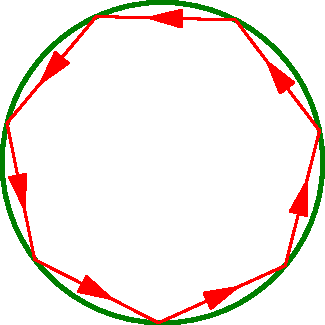
\includegraphics[width=4.5cm]{./Cbillard_4.pdf}}\hspace{1cm}
  \subfloat[Cas $\alpha = \frac{13\pi}{14}$]{\label{fig:Cbillard_5} \includegraphics[width=4.5cm]{./Cbillard_5.pdf}}
  \caption{Question \ref{exples}}
\end{figure}

\item On peut ramener $M_k$ au point d'affixe $1$ par une rotation. Les images de $M_{k+1}$ et $M_{k-1}$ par cette même rotation sont alors $\frac{z_{k+1}}{z_k}$ et $\frac{z_{k-1}}{z_k}$. La symétrie de la figure étant conservée par rotation, les images sont symétriques par rapport à l'axe réel donc
\begin{displaymath}
  \frac{z_{k+1}}{z_k} = \overline{\left( \frac{z_{k-1}}{z_k}\right) }
\Rightarrow
z_{k+1} = \frac{z_k}{\overline{z_k}}\, \overline{z_{k-1}}
\end{displaymath}
Si $z_k=e^{i\beta}z_{k-1}$, on en tire
\begin{displaymath}
  z_{k+1} = \frac{e^{i\beta} z_{k-1}}{e^{-i \beta} \overline{z_{k-1}}} \, \overline{z_{k-1}} = e^{2i\beta} z_{k-1} = e^{i\beta} z_k
  \Rightarrow z_k = e^{ik\beta} z_0
\end{displaymath}
à partir du calcul de $z_1$.
\end{enumerate}
